\documentclass[oneside,senior,etd]{BYUPhysForDegree}
% \documentclass[etd]{BYUPhysForDegree}

\usepackage[utf8]{inputenc}
\usepackage{rotating} 

% \usepackage[russian]{babel}
\usepackage[T2A]{fontenc}
\usepackage[russian]{babel}

\usepackage{amsfonts} % Пакеты для математических символов и теорем
\usepackage{amstext}
\usepackage{amssymb}
\usepackage{amsthm}
\usepackage{graphicx} % Пакеты для вставки графики
\usepackage{subfig}
\usepackage{color}
\usepackage[unicode, breaklinks]{hyperref}
\usepackage[nottoc]{tocbibind} % Для того, чтобы список литературы отображался в оглавлении
% \usepackage{algorithmic} % Для записи алгоритмов в псевдокоде
\usepackage{algorithm}
\usepackage{verbatim} % Для вставок заранее подготовленного текста в режиме as-is
\usepackage{listings}
\usepackage{float}
% \usepackage[space]{cite}

\usepackage{algpseudocode} 

\usepackage{longtable}

\usepackage{ragged2e}
\usepackage{xltabular}

% \usepackage[margin=1.0in]{geometry}
\usepackage{pgfgantt}
\usepackage{subfig}
% \usepackage{subcaption}

% \usepackage{lscape}

\usepackage{enumitem}
\usepackage{mathtools}

\DeclarePairedDelimiter\ceil{\lceil}{\rceil}
\DeclarePairedDelimiter\floor{\lfloor}{\rfloor}


% \usepackage{pgfplots}
\usepackage{array}
% \usepackage{longtable}
\usepackage{indentfirst}
% \usepackage[margin=.70in]{geometry}
% \usepackage{tabularx}
% \usepackage{polyglossia}  
% \usepackage{setspace}
% \usepackage{tocloft}
% \usepackage{algpseudocode}

% \usepackage[maxbibnames=99]{biblatex}
\usepackage{diagbox}
\usepackage[table]{xcolor}

\usepackage{commath}
\newcommand\Tau{\mathcal{T}}
\newcommand{\R}{\mathbb{R}}
\usepackage{color}
% \usepackage[colorinlistoftodos, prependcaption]{todonotes}
\usepackage{multirow}
\newcommand*{\MyIndent}{\hspace*{0.2cm}}%

\renewcommand\tabularxcolumn[1]{m{#1}}

\Chair{Кафедра автоматизации систем вычислительных комплексов}
\Lab{~}
\Year{2026}
  \Month{Октябрь}
  \City{Москва}
  \AuthorText{Автор}
  \Author{Басалов Ярослав Александрович}
  \AuthorEng{Basalov Iaroslav}
  \AcadGroup{м621}
  % Если вы не Пупкин Василий Иванович, то скопируйте себе этот проект через меню и уже потом правьте
  
  \TitleTop{Задание по курсу}
  \TitleMiddle{«Суперкомпьютерное моделирование и технологии»}
  \TitleBottom{} % leave empty if you don't need it
  % \TitleTopEng{Workload distribution to heterogeneous processors}
  \TitleTopEng{Workload distribution to heterogeneous processors}
  \TitleMiddleEng{considering critical path duration}
  % \TitleBottomEng{} % leave empty if you don't need it  
  \TitleBottomEng{} % leave empty if you don't need it  
  % \docname{ВЫПУСКНАЯ КВАЛИФИКАЦИОННАЯ  РАБОТА}
  % \docname{Реферат}
  \docname{Задание 2, Вариант 5}
  %\docname{Магистерская диссертация}
  \Advisor{Басалов Ярослав Александрович}  
  \AdvisorDegree{студент м221 группы}
  % \Consultant{}
  % \ConsultantDegree{}
  
\Abstract{В работе рассматривается задача распределения вычислительной нагрузки (графа работ) по неоднородным процессорам с учетом как суммарных длительностей работ на процессорах, так и длительности критического пути в графе работ. По результатам обзора не выявлено существующих алгоритмов распределения нагрузки, учитывающих оба этих критерия в случае неоднородных процессоров. Для ускорения расчета длительности критического пути предложен переход к транзитному графу работ с сохранением этой длительности. Разработан и реализован генетический алгоритм решения рассматриваемой задачи, работающий с транзитным графом.}
% \makepreliminarypages
\AbstractEng{The paper addresses the problem of workload distribution (task graph) to heterogeneous processors, considering both the total task durations on the processors and the critical path duration in the task graph. The review found no existing workload distribution algorithms that account for both criteria in the case of heterogeneous processors. To expedite the calculation of the critical path duration, a transition to a transit task graph while preserving this duration is proposed. A genetic algorithm has been developed and implemented to solve the problem using the transit graph.}
% \AbstractEng{}


%%%% DON'T change this. It is here because .sty does not support cyrillic cp properly %%%%
\University{Московский государственный университет имени М.В.Ломоносова}
\Faculty{Факультет вычислительной математики и кибернетики}
\GrText{гр.}
\AdvisorText{Выполнил}
% \ConsultantText{Научный консультант}
\AbstractText{Аннотация}

\begin{document}
\fixmargins
\makepreliminarypages

% \oneandhalfspace

% \resizebox{\textwidth}{!}{\tableofcontents}

\tableofcontents
\thispagestyle{empty} % ???

% 
\section*{Введение}
\addcontentsline{toc}{section}{Введение}
% \addcontentsline{toc}{section}{\protect\numberline{}Введение}
\label{sec:Chapter0} \index{Chapter0}

 	
В качестве модельной задачи предлагается задача для трехмерного гиперболического уравнения в области, представляющей из себя прямоугольный параллелепипед.
Индивидуальные варианты заданий отличаются типом граничных условий.
Данное уравнение часто применяется в теории тепло и массопереноса, гидро и аэромеханике, электростатике.
Поэтому поиск решения данный задачи в различных областях является весьма актуальным.


Задание необходимо выполнить на следующих ПВС Московского университета:
\begin{enumerate}
    \item IBM Polus \cite{Polus}.
\end{enumerate}
 % Введение
\section{Математическая постановка дифференциальной задачи}
\label{sec:Chapter1} \index{Chapter1}
Рассматривается трёхмерная замкнутая область
\[
\Omega = [0 \leq x \leq L_x] \times [0 \leq y \leq L_y] \times [0 \leq z \leq L_z]
\]
для $(0 < t \leq T]$ требуется найти решение $u(x, y, z, t)$ уравнения в частных производных
\begin{align}
    \frac{\partial^2 u}{\partial t^2} = \Delta u \label{equation:1}
\end{align} 
с начальными условиями
\begin{align}
    \left.u\right|_{t=0} = \varphi(x,y,z), \label{equation:2}\\
    \left.\frac{\partial u}{\partial t}\right|_{t=0} = 0, \label{equation:3}
\end{align} 
при условии, что на границах области заданы однородные граничные условия первого рода
\begin{align}
    u(0, y, z, t) = 0,
    \qquad
    u(L_x, y, z, t) = 0,
    \label{equation:4}
    \\
    u(x, 0, z, t) = 0,
    \qquad
    u(x, L_y, z, t) = 0,
    \label{equation:5}
    \\
    u(x, y, 0, t) = 0,
    \qquad
    u(x, y, L_z, t) = 0,
    \label{equation:6}
\end{align}
либо периодические граничные условия 
\begin{align}
    u(0, y, z, t) = u(L_x, y, z, t),
    \qquad
    u_x(0, y, z, t) = u_x(L_x, y, z, t),
    \label{equation:7}
    \\
    u(x, 0, z, t) = u(x, L_y, z, t),
    \qquad
    u_y(x, 0, z, t) = u_y(x, L_y, z, t),
    \label{equation:8}
    \\
    u(x, y, 0, t) = u(x, y, L_z, t),
    \qquad
    u_z(x, y, 0, t) = u_z(x, y, L_z, t).
    \label{equation:9}
\end{align}
Конкретная комбинация граничных условий определяется индивидуальным вариантом задания (см. п. \ref{sec:Chapter4})
 % Формальная постановка задачи
\section{Численный метод решения задачи}
\label{sec:Chapter2} \index{Chapter2}
Содержание данного пункта основано на материале книги \cite{Chymi}.

Для численного решения задачи введем на $\Omega$ сетку $\omega_{h\tau} = \overline{\omega}_h \times \omega_\tau$, где

\[
    T = T_0,
\]
\[
    L_x = L_{x0}, L_y = L_{y0}, L_z = L_{z0}
\]
\[
    \overline{\omega}_h = \{\left(x_i=ih_x, y_j=jh_y, z_k=kh_z\right), i,j,k=0,1,\dots,N, h_xN=L_x,h_yN=L_y,h_zN=L_z\},
\]
\[
    \omega_\tau = \{t_n=n\tau,n=0,1,\dots,K,\tau K=T\}.
\]
Через $\omega_{h}$ обозначим множество внутренних, а через $\gamma_{h}$ множество граничных узлов сетки $\overline{\omega}_{h}$.

Для аппроксимации исходного уравнения (\ref{equation:1}) c однородными граничными условиями (\ref{equation:4})--(\ref{equation:6}) и начальными условиями (\ref{equation:2})--(\ref{equation:3}) воспользуемся следующей системой уравнений:
\[
    \frac{
        u^{n+1}_{ijk}
        -
        2 u^{n}_{ijk}
        +
        u^{n-1}_{ijk}
    }
    {
        \tau^2
    }
    =
    \Delta_h u^{n},
    \qquad
    (x_i,y_j,z_k)\in \omega_h,
    \qquad
    n = 1,2,\dots,K-1,
\]
Здесь \(\Delta_h\) — семиточечный разностный аналог оператора Лапласа:
\[
\Delta_h u^{n}
=
\frac{
        u^{n}_{i-1,j,k}
        -
        2u^{n}_{i,j,k}
        +
        u^{n}_{i+1,j,k}
    }
    {h^2}
+
\frac{
        u^{n}_{i,j-1,k}
        -
        2u^{n}_{i,j,k}
        +
        u^{n}_{i,j+1,k}
    }
    {h^2}
+
\frac{
        u^{n}_{i,j,k-1}
        -
        2u^{n}_{i,j,k}
        +
        u^{n}_{i,j,k+1}
    }
    {h^2}.
\]
Приведенная выше разностная схема является явной -- значения \(u^{n+1}_{ijk}\) на \((n+1)\)-м шаге можно явным образом выразить через значения на предыдущих слоях.

Для начала счета (т.е. для нахождения \(u^{2}_{ijk}\)) должны быть заданы значения \(u^{0}_{ijk}\), \(u^{1}_{ijk}\), \((x_i,y_j,z_k) \in \omega_{h}\).
Из условия (\ref{equation:2}) имеем
\begin{align}
    u^{0}_{ijk}
    =
    \varphi(x_i,y_j,z_k),
    \qquad
    (x_i,y_j,z_k) \in \omega_{h}.
    \label{equation:10}
\end{align}
Простейшая замена начального условия (\ref{equation:3}) уравнением \((u^{1}_{ijk}-u^{0}_{ijk})/\tau=0\) имеет лишь первый порядок аппроксимации по \(\tau\).
Аппроксимацию второго порядка по \(\tau\) и \(h\) дает разностное уравнение
\begin{align}
    \dfrac{u^{1}_{ijk}-u^{0}_{ijk}}{\tau}
    =
    \dfrac{\tau}{2}\Delta_h\varphi(x_i,y_j,z_k),
    \qquad
    (x_i,y_j,z_k) \in \omega_{h}.
    \label{equation:11}
    \\
    u^{1}_{ijk}
    =
    u^{0}_{ijk}+\dfrac{\tau^2}{2}\Delta_h\varphi(x_i,y_j,z_k)
    \label{equation:12}
\end{align}

Разностная аппроксимация для периодических граничных условий выглядит следующим образом
\[
    u^{n+1}_{0jk}=u^{n+1}_{Njk},
    \qquad
    u^{n+1}_{1jk}=u^{n+1}_{N+1jk},
\]
\[
    u^{n+1}_{i0k}=u^{n+1}_{iNk},
    \qquad
    u^{n+1}_{i1k}=u^{n+1}_{iN+1k},
\]
\[
    u^{n+1}_{ij0}=u^{n+1}_{ijN},
    \qquad
    u^{n+1}_{ij1}=u^{n+1}_{ijN+1},
\]
\(i,j,k=0,1,\dots,N\).

Для вычисления значений \(u^0, u^1, \in \gamma_{h}\) допускается использование аналитического значения \(u\), которое задается в программе еще для вычисления погрешности решения задачи.
 %  Численный метод решения задачи 
\section{Программная реализация}
\label{sec:Chapter3} \index{Chapter3}
Требуется реализовать блочное разбиение области между процессами, поскольку в этом случае предполагается меньше межпроцессорных коммуникаций, по сравнению с ленточным.

\captionsetup[subfloat]{labelformat=empty}
\begin{figure}[H]
    \centering
    \subfloat[Ленточное разбиение 3d]{%
        \raisebox{-0.5\height}{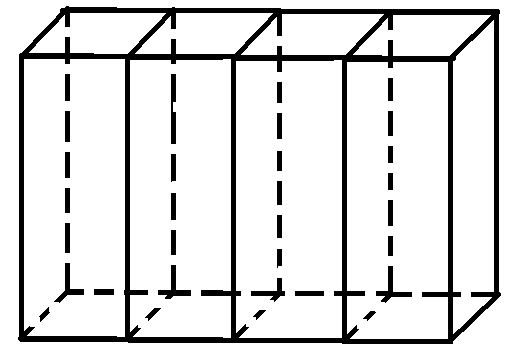
\includegraphics[width=.49\linewidth]{./images/0.png}}%
    }
    \hfill
    \subfloat[Блочное разбиение 3d]{%
        \raisebox{-0.5\height}{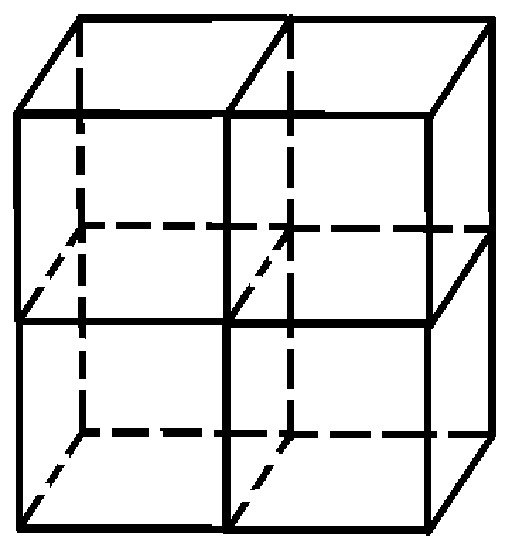
\includegraphics[width=.49\linewidth]{./images/1.png}}%
    }
    \caption{Виды разбиений 3d}
    \label{fig:1}
\end{figure}

Число областей, на которое необходимо произвести разбиение может быть произвольным, как четным, так и нечетным. 

На рисунке \ref{fig:1} изображен схематично двумерный ленточный и блочный вариант разбиения квадратной области на 8 частей. 

В случае ленточного разбиения получаем \(S_{strip}=8L\) межпроцессорных коммуникаций.
В блочном случае \(S_{block}=8(L/2)+4(L/4)=5L\) коммуникаций, то есть в 1.6 раз меньше.
С ростом числа разбиений (и процессов, соответственно) это число будет только увеличиваться.
Данные рассуждения можно обобщить и на трехмерный случай.

\begin{figure}[H]
    \centering
    \subfloat[Ленточное разбиение]{%
        \raisebox{-0.5\height}{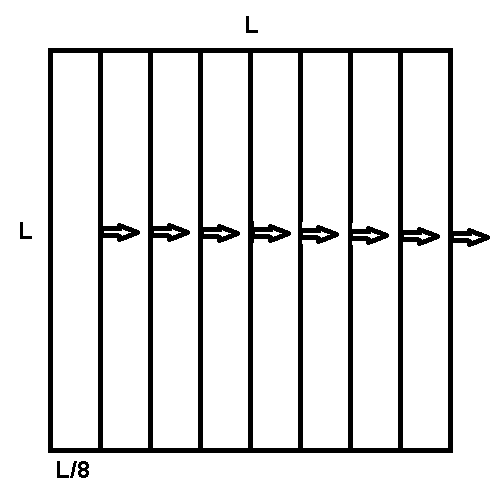
\includegraphics[width=.49\linewidth]{./images/2.png}}%
    }
    \hfill
    \subfloat[Блочное разбиение]{%
        \raisebox{-0.5\height}{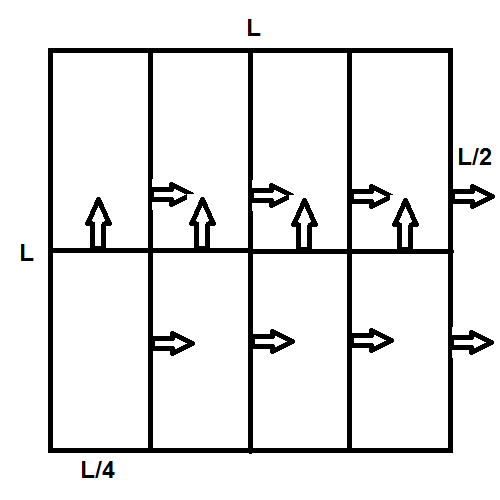
\includegraphics[width=.49\linewidth]{./images/3.png}}%
    }
    \caption{Виды разбиений}
    \label{fig:2}
\end{figure}
Таким образом, алгоритм решения задачи, выглядит следующим образом:
\begin{enumerate}
    \item Исходя из варианта, расчитывается точное аналитическое решение \(u_{analytical}\) в узлах сетки.
    \item Проводим разбиение области \(\Omega\) между процессами.
    \item Фиксируем временной слой (начиная с \(0\)). 
    \item Используя формулы (\ref{equation:10}) и (\ref{equation:12}). находим значения \(u^0\) и \(u^1\).
    \item Пользуясь найденными \(u^0\) и \(u^1\) и разностным представлением уравнения (\ref{equation:1}), находим значения \(u\) в локальной области разбиения. 
    \item Передаем посчитанные граничные значения блокам-соседям.
    \item Повторяем шаги 5--6 для внутренних блоков.
    \item Определяем максимальную погрешность на сетке между посчитанным и аналитическим решением.
    \item Переходим на следующий слой по времени и повторяем шаги 2--9.
\end{enumerate}


\lstset{
backgroundcolor=\color{gray!10},
frame=single,
basicstyle=\ttfamily\small,
breaklines=true,
columns=fullflexible
}
Реализация данного алгоритма была написана на языке C++ и выложена на GitHub (https://github.com/Marilius/edu-cmc-skmodel26).
Для компиляции и запуска использовались подобные команды (версия с OpenMP):
\begin{lstlisting}[language=Bash, caption=Пример запуска с OpenMP]
g++ -O2 -fopenmp -std=c++11 src/main.cpp -o solver.out
mpisubmit.pl -t 8 solver.out --stdout std.out --stderr std.err \
-- 128 20 1. 1. 1. 0.01
\end{lstlisting}

% TODO
% Lx = Ly = Lz = 1, Lx =
% Ly = Lz =  % Программная реализация
\section{Вариант задания}
\label{sec:Chapter4} \index{Chapter4}
Индивидуальные варианты заданий отличаются комбинацией граничных условий.
% Варианты приведены в следующей таблице (1Р -- условие первого рода, П -- периодическое условие) 1. 

В текущей работе рассматривается вариант 5:
\begin{itemize}
    \item $
        u_{analytical}
        =
        sin \left( \frac{2\pi}{L_x}x \right)
        \cdot
        sin \left( \frac{2\pi}{L_y}y \right)
        \cdot
        sin \left( \frac{2\pi}{L_z}z \right)
        \cdot
        cos \left( a_t \cdot t + 4\pi \right),
        a_t
        =
        \pi \sqrt{
            \dfrac{4}{L^2_x}
            +
            \dfrac{1}{L^2_y}
            +
            \dfrac{1}{L^2_z}
        }
    $,
    \item \(x\) -- периодическое условие (\ref{equation:7}),
    \item \(y\) -- условие первого рода (\ref{equation:5}),
    \item \(z\) -- условие первого рода (\ref{equation:6}).
\end{itemize}

Функция \(u_{analytical}\) напрямую зависит от введенных \(L_x\), \(L_y\), \(L_z\), которые являются входными аргументами программы.
Функция \(\varphi(x, y, z)\) зависит напрямую от \(u_{analytical}\) (\ref{equation:2}). % Варианты задания
% \include{Algo} % Описание сведение к задачи ВКР части
\section{Исследование масштабируемости}
\label{sec:Chapter5} \index{Chapter5}

\subsection{Результаты расчетов для OpenMP программы}
\begin{table}[ht]
    \begin{tabular}{|c|c|c|c|}
        \hline
        \makecell[c]{Число OpenMP-нитей\\ / послед. алгоритм} & Размер сетки & Время решения & Ускорение \\
        \hline
        serial & \(128^3\) & 12.38718873 & 1.0 \\
        1 & \(128^3\) & 11.906204419 & 1.0403977870758243 \\
        2 & \(128^3\) & 6.179221872 & 2.0046518779541245 \\
        4 & \(128^3\) & 3.195486474 & 3.876464141152863 \\
        8 & \(128^3\) & 2.020456917 & 6.1308848636043445 \\
        \hline
        serial & \(256^3\) & 98.77836788 & 1.0 \\
        1 & \(256^3\) & 94.707646745 & 1.0429819689846207 \\
        2 & \(256^3\) & 48.758578746 & 2.0258664304915466 \\
        4 & \(256^3\) & 25.047241724 & 3.943682460865606 \\
        8 & \(256^3\) & 15.251786104 & 6.476511485700285 \\
        \hline
        serial & \(512^3\) & 787.55294798 & 1.0 \\
        1 & \(512^3\) & 754.75414806 & 1.043456269838735 \\
        2 & \(512^3\) & 384.922989328 & 2.0460013296553496 \\
        4 & \(512^3\) & 199.994196498 & 3.9378790073434744 \\
        5 & \(512^3\) & 122.05060391 & 6.4526755521893255 \\
        \hline
    \end{tabular}
    \caption{Время решения, \(L_x=L_y=L_z=1\)}
    \label{tab1}
\end{table}

\begin{figure}[ht]
    \centering
    \begin{tikzpicture}
        \begin{axis}[
            width=12cm,
            height=8cm,
            xlabel={Число OpenMP-нитей},
            ylabel={Время выполнения, с},
            legend pos=north east,
            grid=major,
            xtick={1,2,4,8}
        ]
        \addplot coordinates {
            (1,11.906204419)
            (2,6.179221872)
            (4,3.195486474)
            (8,2.020456917)
        };
        \addlegendentry{$128^3$}
        \addplot coordinates {
            (1,94.707646745)
            (2,48.758578746)
            (4,25.047241724)
            (8,15.251786104)
        };
        \addlegendentry{$256^3$}
        \addplot coordinates {
            (1,754.75414806)
            (2,384.922989328)
            (4,199.994196498)
            (8,122.05060391)
        };
        \addlegendentry{$512^3$}
        \end{axis}
    \end{tikzpicture}
    \caption{
        Время выполнения OpenMP-реализации при различных размерах сетки
        \newline
        \centering\(L_x=L_y=L_z=1\)
    }
    \label{fig:tab1:time}
\end{figure}

\begin{figure}[ht]
    \centering
    \begin{tikzpicture}
        \begin{axis}[
            width=12cm,
            height=8cm,
            xlabel={Число OpenMP-нитей},
            ylabel={Ускорение},
            legend pos=north west,
            grid=major,
            xtick={1,2,4,8}
        ]
        \addplot coordinates {
            (1,1.0403977870758243)
            (2,2.0046518779541245)
            (4,3.876464141152863)
            (8,6.1308848636043445)
        };
        \addlegendentry{$128^3$}
        \addplot coordinates {
            (1,1.0429819689846207)
            (2,2.0258664304915466)
            (4,3.943682460865606)
            (8,6.476511485700285)
        };
        \addlegendentry{$256^3$}
        \addplot coordinates {
            (1,1.043456269838735)
            (2,2.0460013296553496)
            (4,3.9378790073434744)
            (8,6.4526755521893255)
        };
        \addlegendentry{$512^3$}
        \end{axis}
    \end{tikzpicture}
    \caption{
        Ускорение OpenMP-реализации при различных размерах сетки
        \newline
        \centering\(L_x=L_y=L_z=1\)
    }
    \label{fig:tab1:speedup}
\end{figure}

\noindent
Последовательный и параллельный варианты программы были скомпилированы с флагом оптимизации -O2.
При любом числе потоков получили проигрыш по сравнению с последовательным вариантом алгоритма.
Компилятор GCC довольно хорошо оптимизирует последовательный код.

\begin{table}[ht]
    \begin{tabular}{|c|c|c|c|}
        \hline
        \makecell[c]{Число OpenMP-нитей\\ / послед. алгоритм} & Размер сетки & Время решения & Ускорение \\
        \hline
        serial & \(128^3\) & 12.371096542 & 1.0 \\
        1 & \(128^3\) & 12.418100815 & 0.9962148581574387 \\
        2 & \(128^3\) & 8.258355857 & 1.4980096227645523 \\
        4 & \(128^3\) & 4.719976269 & 2.6210082078698687 \\
        8 & \(128^3\) & 2.868507856 & 4.312728834304437 \\
        \hline
        serial & \(256^3\) & 98.502743678 & 1.0 \\
        1 & \(256^3\) & 98.622051571 & 0.998790251357587 \\
        2 & \(256^3\) & 53.337296491 & 1.8467892105221553 \\
        4 & \(256^3\) & 32.507485622 & 3.030155725465786 \\
        8 & \(256^3\) & 15.746087913 & 6.255696286102655 \\
        \hline
        serial & \(512^3\) & 785.029544667 & 1.0 \\
        1 & \(512^3\) & 753.413243477 & 1.0419640900445164 \\
        2 & \(512^3\) & 399.393005665 & 1.9655565659190875 \\
        4 & \(512^3\) & 227.560406705 & 3.4497633223370014 \\
        5 & \(512^3\) & 139.734042225 & 5.618026446289616 \\
        \hline
    \end{tabular}
    \caption{Время решения, \(L_x=L_y=L_z=\pi\)}
    \label{tab2}
\end{table}

\begin{figure}[ht]
    \centering
    \begin{tikzpicture}
        \begin{axis}[
            width=12cm,
            height=8cm,
            xlabel={Число OpenMP-нитей},
            ylabel={Время выполнения, с},
            legend pos=north east,
            grid=major,
            xtick={1,2,4,8}
        ]
        \addplot coordinates {
            (1,12.418100815)
            (2,8.258355857)
            (4,4.719976269)
            (8,2.868507856)
        };
        \addlegendentry{$128^3$}
        \addplot coordinates {
            (1,98.622051571)
            (2,53.337296491)
            (4,32.507485622)
            (8,15.746087913)
        };
        \addlegendentry{$256^3$}
        \addplot coordinates {
            (1,753.413243477)
            (2,399.393005665)
            (4,227.560406705)
            (8,139.734042225)
        };
        \addlegendentry{$512^3$}
        \end{axis}
    \end{tikzpicture}
    \caption{
        Время выполнения OpenMP-реализации при различных размерах сетки
        \newline
        \centering\(L_x=L_y=L_z=\pi\)
    }
    \label{fig:tab2:time}
\end{figure}

\begin{figure}[ht]
    \centering
    \begin{tikzpicture}
        \begin{axis}[
            width=12cm,
            height=8cm,
            xlabel={Число OpenMP-нитей},
            ylabel={Ускорение},
            legend pos=north west,
            grid=major,
            xtick={1,2,4,8}
        ]
        \addplot coordinates {
            (1,0.9962148581574387)
            (2,1.4980096227645523)
            (4,2.6210082078698687)
            (8,4.312728834304437)
        };
        \addlegendentry{$128^3$}
        \addplot coordinates {
            (1,0.998790251357587)
            (2,1.8467892105221553)
            (4,3.030155725465786)
            (8,6.255696286102655)
        };
        \addlegendentry{$256^3$}
        \addplot coordinates {
            (1,1.0419640900445164)
            (2,1.9655565659190875)
            (4,3.4497633223370014)
            (8,5.618026446289616)
        };
        \addlegendentry{$512^3$}
        \end{axis}
    \end{tikzpicture}
    \caption{
        Ускорение OpenMP-реализации при различных размерах сетки
        \newline
        \centering\(L_x=L_y=L_z=\pi\)
    }
    \label{fig:tab2}
\end{figure}




\begin{figure}
    \centering
    \begin{tikzpicture}
        \begin{axis}[
            width=12cm,
            height=7cm,
            xlabel={Время},
            ylabel={Ошибка},
            grid=major,
            legend pos=north west,
            xmin=0,
            xmax=1,
            title={Максимальная абсолютная ошибка},
        ]

        \addplot table[
            x expr=\coordindex*0.02,
            y index=0
        ] {../results/run_logs_L1/max_errors.txt};
        \addlegendentry{\(L_x=L_y=L_z=1\)}

        \addplot table[
            x expr=\coordindex*0.02,
            y index=0
        ] {../results/run_logs_LPI/max_errors.txt};
        \addlegendentry{\(L_x=L_y=L_z=\pi\)}

        \end{axis}
    \end{tikzpicture}
    \caption{
        Размер сетки = \(128^3\), 50 шагов по времени
    }
    \label{fig:error}
\end{figure}
 % Исследование масштабируемости
\section*{Заключение}
\addcontentsline{toc}{section}{Заключение}
% \label{sec:Chapter1} \index{Chapter1}
TODO % Заключение

% \nocite{*}
\bibliographystyle{gost71u} % Для соответствия требованиям об оформлении списка литературы
\bibliography{references}

% \include{Appendix}

\end{document}
